\documentclass[12pt]{scrartcl}
\usepackage[sexy]{james}
\usepackage[noend]{algpseudocode}
\setlength {\marginparwidth}{2cm}
\usepackage{answers}
\usepackage{array}
\usepackage{tikz}
\newenvironment{allintypewriter}{\ttfamily}{\par}
\usepackage{listings}
\usepackage{xcolor}
\usetikzlibrary{arrows.meta}
\usepackage{color}
\usepackage{mathtools}
\newcommand{\U}{\mathcal{U}}
\newcommand{\E}{\mathbb{E}}
\usetikzlibrary{arrows}
\Newassociation{hint}{hintitem}{all-hints}
\renewcommand{\solutionextension}{out}
\renewenvironment{hintitem}[1]{\item[\bfseries #1.]}{}
\renewcommand{\O}{\mathcal{O}}
\declaretheorem[style=thmbluebox,name={Chinese Remainder Theorem}]{CRT}
\renewcommand{\theCRT}{\Alph{CRT}}
\setlength\parindent{0pt}
\usepackage{sansmath}
\usepackage{pgfplots}

\usetikzlibrary{automata}
\usetikzlibrary{positioning}  %                 ...positioning nodes
\usetikzlibrary{arrows}       %                 ...customizing arrows
\newcommand{\eqdef}{=\vcentcolon}
\newcommand{\tr}{{\rm tr\ }}
\newcommand{\im}{{\rm Im\ }}
\newcommand{\spann}{{\rm span\ }}
\newcommand{\Col}{{\rm Col\ }}
\newcommand{\Row}{{\rm Row\ }}
\newcommand{\dint}{\displaystyle\int}
\newcommand{\dt}{\ {\rm d }t}
\newcommand{\PP}{\mathbb{P}}
\newcommand{\horizontal}{\par\noindent\rule{\textwidth}{0.4pt}}
\usepackage[top=3cm,left=3cm,right=3cm,bottom=3cm]{geometry}
\newcommand{\mref}[3][red]{\hypersetup{linkcolor=#1}\cref{#2}{#3}\hypersetup{linkcolor=blue}}%<<<changed

\tikzset{node distance=4.5cm, % Minimum distance between two nodes. Change if necessary.
         every state/.style={ % Sets the properties for each state
           semithick,
           fill=cyan!40},
         initial text={},     % No label on start arrow
         double distance=4pt, % Adjust appearance of accept states
         every edge/.style={  % Sets the properties for each transition
         draw,
           ->,>=stealth',     % Makes edges directed with bold arrowheads
           auto,
           semithick}}


% Start of document.
\newcommand{\sep}{\hspace*{.5em}}

\pgfplotsset{compat=1.18}
\begin{document}
\title{MATH403: Homework 1}
\author{James Zhang\thanks{Email: \mailto{jzhang72@terpmail.umd.edu}}}
\date{\today}

\definecolor{dkgreen}{rgb}{0,0.6,0}
\definecolor{gray}{rgb}{0.5,0.5,0.5}
\definecolor{mauve}{rgb}{0.58,0,0.82}

\lstset{frame=tb,
  language=Java,
  aboveskip=3mm,
  belowskip=3mm,
  showstringspaces=false,
  columns=flexible,
  basicstyle={\small\ttfamily},
  numbers=left,
  numberstyle=\tiny\color{gray},
  keywordstyle=\color{blue},
  commentstyle=\color{dkgreen},
  stringstyle=\color{mauve},
  breaklines=true,
  breakatwhitespace=true,
  tabsize=3
}

\maketitle

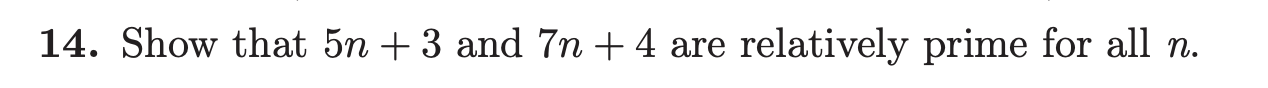
\includegraphics[width=11cm]{14.png}

\begin{proof}
  Two numbers are relatively prime if the greatest common divisor between then is $1$. By Bezout's Lemma, 
  we want to find two integers $x, y$ such that $(5n + 3)x + (7n + 4)y = 1$. Note that we can rewrite this as 
  \[(5x + 7y)n + (3x + 4y) = 1\]
  which yields the following system of equations 
  \[\begin{cases}
    5x + 7y = 0\\
    3x + 4y = 1
  \end{cases}\]
  which yields $x = 7, y = -5$. Therefore, since $(7n + 4) * -5 + (5n + 3) * 7 = -1$, we conclude that 
  $GCD(5n + 3, 7n + 4) = 1$ and so $5n + 3$ and $7n + 4$ are relatively prime.
\end{proof}

\newpage

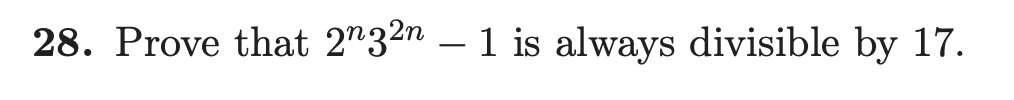
\includegraphics[width=11cm]{28.png}

\begin{proof}
  We will prove the following using strong induction. 

  Base case: $n = 0 \implies 2^n3^{2n} - 1 = 1 - 1 = 0$ is divisible by $17$. If the set of naturals doesn't include $0$, $n = 1 = 2^1 3^{2} - 1 = 18 - 1 = 17$, which is trivially satisfied by $17$. 

  \hfill
  
  Inductive hypothesis: assume $2^n 3^{2n} - 1$ is divisible by $17$ for all $n \leq k$.

  Therefore, for all $n \leq k$, we can write express $2^n 3^{2n} = 17x + 1, x \in \ZZ$

  \hfill
  
  Inductive case: we seek to show that $2^{k+1} 3^{2(k+1)} - 1$ is divisible by $17$. Equivalently, we want to show 
  that there exists a $x \in \ZZ$ such that $2^{k+1} 3^{2(k+1)}  - 1 = 17x$. Note that
  \[2^{k+1} 3^{2(k+1)} - 1 = (2 \cdot 3^2)(2^k 3^{2k}) - 1\]
  Further note that by our inductive hypothesis, $\exists \ y \in \ZZ$ such that $2^k 3^{2k} + 1 = 17y$. By direct 
  substitution, 
  \[18(17y + 1) - 1 = 306y + 18 - 1 = 306y + 17 = 17(18y + 1)\]
  Let $x = 18y + 1 \in \ZZ$ and therefore we have expressed $2^{k+1} 3^{2(k+1)} = 17x$ and so 
  $2^n3^{2n} - 1$ is always divisible by $17$ for all $n$. 
\end{proof}

\newpage 

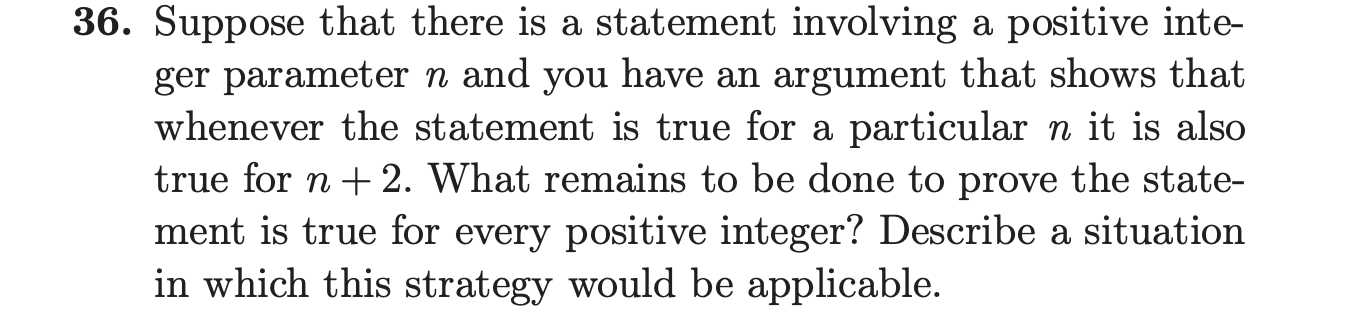
\includegraphics[width=13cm]{36.png}

\begin{proof}[Solution]
  To prove that the statement is true for every positive integer, you have to explicitly show that 
  it is true for $n = 1$ and $n = 2$ because for these two examples, you cannot use the above argument here 
  because $n - 2$ is $-1$ and $0$, respectively. These numbers are not positive integers, and 
  so the above argument cannot be applied. This idea naturally leads to the mathematical idea of induction, and these 
  base cases provide the foundation for the induction process.

  \hfill

  This strategy of inductively proving an statement is particularly useful when the statement involves 
  properties that are either periodic or depend on even or odd integers. It can also be 
  useful for proofs related to sequences defined using recurrence relations. 
\end{proof}

\newpage

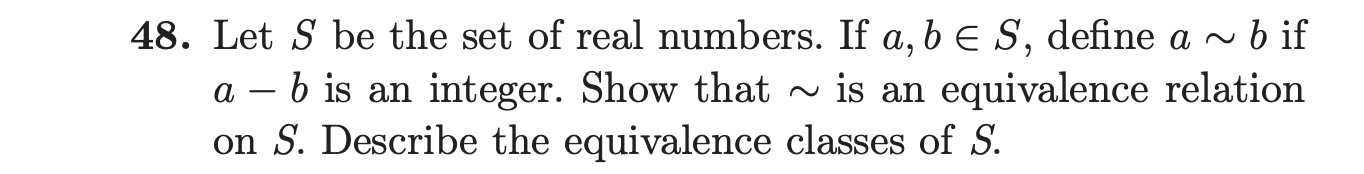
\includegraphics[width=12cm]{48.png}

\begin{proof}
Let $R \subset \RR \times \RR$. First, let us show that this relation $\sim$ is an equivalence relation. 
For any $a \in \RR$, $a - a = 0 \in \ZZ$, so $a \sim a$ for all $a \in \RR$ and reflexivity 
is satisfied. For symmetry, note that if $a \sim b$, then $a - b \in \ZZ$ but also 
$b -a = -(a-b) \in \ZZ$ and so $b \sim a$, so symmetry is satisfied. Finally, suppose $a\sim b$
such that $a - b = m \in \ZZ$ and $b \sim c = n \in \ZZ$. Since $(a-c) = (a-b) + (b-c) = m + n \in ZZ$ then 
$a-c\in \ZZ$ and so $a \sim c$. In this original relation, the equivalence class for a number $a \in \RR$ is 
\[[a] = \{x \in \RR \ | \ x \sim a\} = \{x \in \RR \ | \ x - a \in \ZZ\}\] 
Here are some example equivalence classes. 

$[0] = [\ldots, -1, 0, 1, \ldots]$

$[\pi] = [\ldots, -\pi, 0, \pi, \ldots]$

$[1.2] = [\ldots, -2.2, -1.2, -0.2, 0.8, 1.8, 2.8, \ldots]$.
\end{proof}

\newpage 

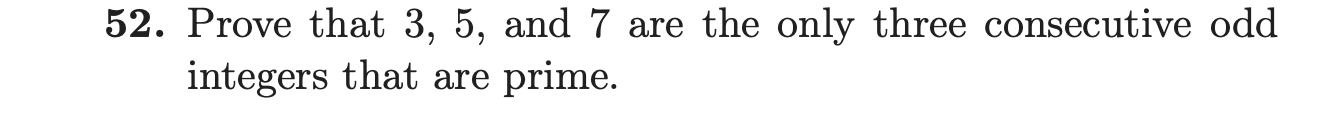
\includegraphics[width=11cm]{52.png}

\begin{proof}
  Assume on the contrary there exists an odd prime number $n > 3$ such that 
  $n, n + 2, n + 4$, the $3$ consecutive odd numbers starting from $n$, are all prime. Consider the number $n$. $n \text{ mod } 3 = 1$ or $2$. 
  It cannot be $0$ because this would contradict the fact that the number is prime, if it is 
  immediately divisible by $3$. 
  
  \hfill

  Case $1$: Suppose $n \text{ mod } 3 = 1$. Then 
  \[(n+2) \text{ mod } 3 = (n \text{ mod } 3 + 2 \text { mod } 3) \text{ mod } 3 = (1 + 2) \text{ mod } 3 = 0\]
  This is a contradiction because $n + 2$ is assumed to be prime, but we have shown that $n + 2$ is divisible by $3$ and therefore not prime. 

  \hfill

  Case $2$: Now suppose $n \text{ mod } 3 = 2$. Then 
  \[(n + 2) \text{ mod } 3 = (n \text{ mod } 3 + 2 \text{ mod } 3) \text{ mod 3} = (2 + 2) \text{ mod } 3 = 1\]
  Thus, $(n + 2) \text{ mod } 3 = 1$ and so $3$ does not divide $n + 2$. However, now consider $n + 4$
  \[(n + 4 \text{ mod } 3) = (n \text { mod } 3 + 4 \text{ mod } 3) \text{ mod 3} = (2 + 1) \text{ mod } 3 = 0\]
  Therefore, $3$ divides $n + 4$ and so by definition, $n + 4$ is not prime, and this is also a contradiction.

  \hfill

  Therefore, there does not exist $3$ consecutive odd integers starting from $n > 3$ that are all prime, 
  and the only example of $3$ consecutive odd integers that are prime is indeed $3, 5, 7$. 
\end{proof}

\end{document}

